

\chapter{Example with picture}

Here we test picture and how this is shown


\section{Picture with subtitle}

\begin{figure}[h]
\noindent \begin{centering}
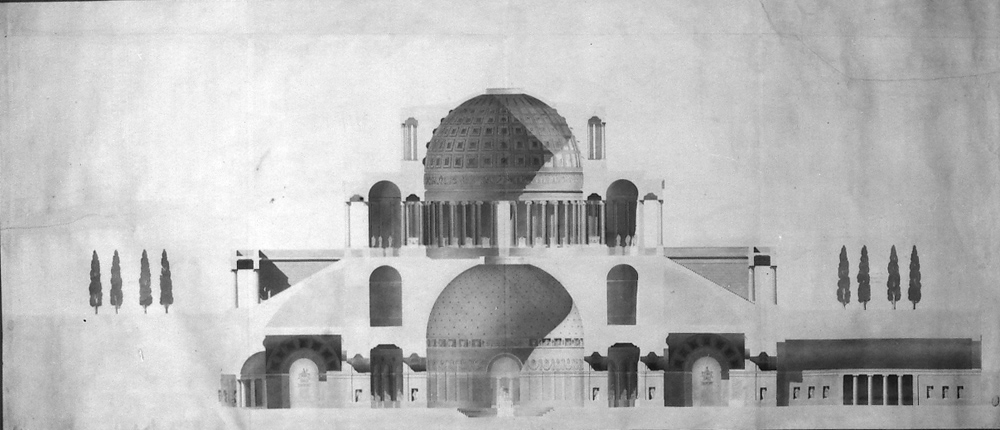
\includegraphics[width=15cm]{images/chapter2/1799_Diplomarbeit_Schnitt}
\par\end{centering}

\protect\caption[Short title which is only displayed in the list of figures]{This is a very long text. Here the picture should be described like this be that you also have an idea of the picture, if only the subtitle read \label{fig:testpicture}}
\end{figure}


In this text, i refer to the above-mentioned picture (see figure \vref{fig:testpicture}). For this, a so called brand has to be inserted in the picture ( in this case: fig:testpicture). As image width is in this document 15cm chosen. This looks very passable in the text out. Try to stay consistent with the widths of the pictures. So 15cm and 10cm for example. This helps the reader and does not interrupt constantly in the reading flow.

\newpage

\section{A section on a new page in the same chapter}